\section{Experiments}
\label{sec:exp}

\subsection{Experimental Setup}

\paragraph{Implementation details.}
For retrieval we use a DINOv3 ViT-B/16 encoder~\cite{dinov3} on normal renderings at four times
the sensor footprint, resized to $224\times224$, and rank references by cosine similarity between
$\ell_2$-normalized class-token features. Coarse alignment uses SuperPoint
keypoints~\cite{superpoint} matched by SuperGlue~\cite{superglue} on the same $4\times$ normal
renderings, with an affine model fitted by RANSAC~\cite{ransac} and a median translation offset
recovered at video resolution. The refinement network is the smallest ReBotNet
variant~\cite{rebotnet} (embedding widths $28/36/48/64$), taking a pair of $240\times320$ frames
plus the three concatenated query normal channels. We train for 20 epochs with AdamW, batch size
8, learning rate $2\times10^{-4}$ with a cosine schedule, and $\lambda = 0.1$; the best checkpoint
by validation PSNR occurs at epoch 18. Training runs on a single RTX 3090 GPU and takes \tbd{}
hours.

\paragraph{Benchmark.}
We create a benchmark for evaluating tactile analogies using the ObjectFolder
dataset~\cite{objectfolder}. For every object we generate a set of tactile normal videos recording
the gel normal changes over time, simulated with the Taxim tactile simulator~\cite{taxim} using a
scaled GelSight Mini calibration at $240\times320$ resolution. Each touch is a 50-frame video at
5\,fps following a press-in-then-withdraw depth schedule. Every touch is accompanied by
view-space renderings of the surface at the sensor pose --- RGB colour, heightmap, surface normal,
curvature and shape index --- at $1\times$, $2\times$ and $4\times$ the sensor footprint. In total
the benchmark comprises 17{,}522 touch locations and 876{,}100 tactile frames across all 1000
ObjectFolder objects. Objects 1--950 form the training split and objects 951--1000 the evaluation
split.

We define two benchmark settings.

\emph{Ground-truth retrieval benchmark.} Each item is a pair of touches --- one designated query,
one designated reference --- with their tactile videos and normal renderings. Because the pairing
is given, this setting isolates the coarse alignment and refinement stages from retrieval error.
We simulate 8 reference and 8 query touches per object, giving 16{,}000 touch locations, with the
query touches perturbed by up to $\pm15^\circ$ of in-plane rotation relative to the references.
The evaluation split contains 400 query touches.

\emph{Full pipeline benchmark.} Here we evaluate the complete pipeline including retrieval. We
collect $K$ touches per object --- on average 15.2 touches on each of 100 objects, 1{,}522
locations in total, with up to $\pm30^\circ$ of rotation jitter --- then hold out $M$ touches as
queries, retrieve against the remaining touches to pick a reference, align, and refine with the
same pre-trained network.

\paragraph{Baselines.}
Since the task is new, we adapt techniques from prior work in tactile perception.

\emph{Tactile-Augmented Radiance Fields (TaRF)}~\cite{tarf} trains a diffusion model that takes
RGB and depth maps as input and outputs a tactile image. We retrain it on the training split of our
ground-truth retrieval benchmark, using the middle frame of each tactile video as the prediction
target. Because its output is a single image rather than a video, we tile the predicted frame to
the length of the reference video.

\emph{Tactile normal quilting}, adapted from Tactile DreamFusion~\cite{tactiledreamfusion}, uses
image quilting to tile the tactile normal of the reference touch across the entire object mesh
surface, renders the view-space normal at the query sensor pose, integrates the normals into a
height field, and renders a tactile video with Taxim~\cite{taxim}.

\emph{Implicit neural representations}, adapted from ObjectFolder~\cite{objectfolder}, train a
NeRF-like implicit representation that takes pixel coordinates and pressing depth as input and
outputs the tactile normal. The representation is fitted per sample on the reference touches and
evaluated at the query locations.

We report PSNR, SSIM and LPIPS, averaged over all frames of all evaluation touches.

\subsection{Performance Comparison}

\subsubsection{Ground-truth retrieval}

%% Ground-truth retrieval benchmark: our method vs. baselines.
%% Numbers from paper_experiments/job1_gt_retrieval/{results.json,table_body.tex}
%% (50 held-out objects 951-1000, 8 touch locations each).
\begin{table}[t]
  \centering
  \small
  \caption{\textbf{Ground-truth retrieval benchmark.} Prediction accuracy averaged over all
    evaluation touches and all frames, with the reference touch supplied by construction so that
    retrieval error is excluded. ``Coarse'' is the transfer obtained from feature-matching
    alignment alone, and ``refined'' additionally applies the refinement network. Arrows indicate
    whether higher ($\uparrow$) or lower ($\downarrow$) is better. Best result in \textbf{bold}.}
  \label{tab:gt_retrieval}
  \begin{tabular}{l c c c}
    \hline
    Method & PSNR $\uparrow$ & SSIM $\uparrow$ & LPIPS $\downarrow$ \\
    \hline
    Tactile normal quilting~\cite{tactiledreamfusion} & 14.58 & 0.7227 & 0.4833 \\
    Implicit neural representation~\cite{objectfolder} & 18.26 & 0.8166 & 0.3821 \\
    \hline
    Ours (coarse transfer)                        & 22.90 & 0.8363 & 0.2102 \\
    Ours (refined)                                & \textbf{31.21} & \textbf{0.9224} & \textbf{0.1085} \\
    \hline
  \end{tabular}
\end{table}


Table~\ref{tab:gt_retrieval} reports quantitative results on the ground-truth retrieval benchmark,
separately for the coarse transfer produced by feature-matching alignment alone and for the final
refined transfer. Fig.~\ref{fig:gt_retrieval} shows qualitative results at a range of touch
locations: for each row we show the reference touch, the reference and query normal renderings,
the coarse transfer, our refined prediction, and the ground-truth query touch.

%% Qualitative results on the ground-truth retrieval benchmark (two columns).
%% The graphic is a 5 x 6 matrix of images -- 5 touch locations (rows) x 6 streams (columns):
%%   1. reference touch, middle frame
%%   2. reference normal render at the reference sensor pose
%%   3. query normal render at the query sensor pose
%%   4. query touch, coarse transfer
%%   5. query touch, refined transfer (ours)
%%   6. ground-truth query touch
%% Columns 2 and 3 show four times the sensor footprint with the sensor's own footprint
%% boxed in red, are drawn on white, and are the only columns with an outline.
%% Graphic: figures/gt_retrieval.png
%% Column headers are baked into the image.
%% Source PDF: log/paper_job06_gt_retrieval_figure/gt_retrieval.pdf (white page, black text)
%% Per-cell PNGs: log/paper_job06_gt_retrieval_figure/assets_pdf/gt_retrieval/
%%   rowN_<object>_<touch>_colM_<stream>.png
%% Rows shown: objects 974/5, 978/4, 969/3, 970/7, 995/5.
%% Built by paper_experiments/06_gt_retrieval_figure/make_gt_figure.py; per-cell PNGs for
%% all 400 evaluation touches remain in
%%   log/paper_job02_gt_retrieval_figure_normalmatch/assets/
%%   named <object>_<touch>_01_ref_touch.png ... _06_gt_query.png
\begin{figure*}[t]
  \centering
  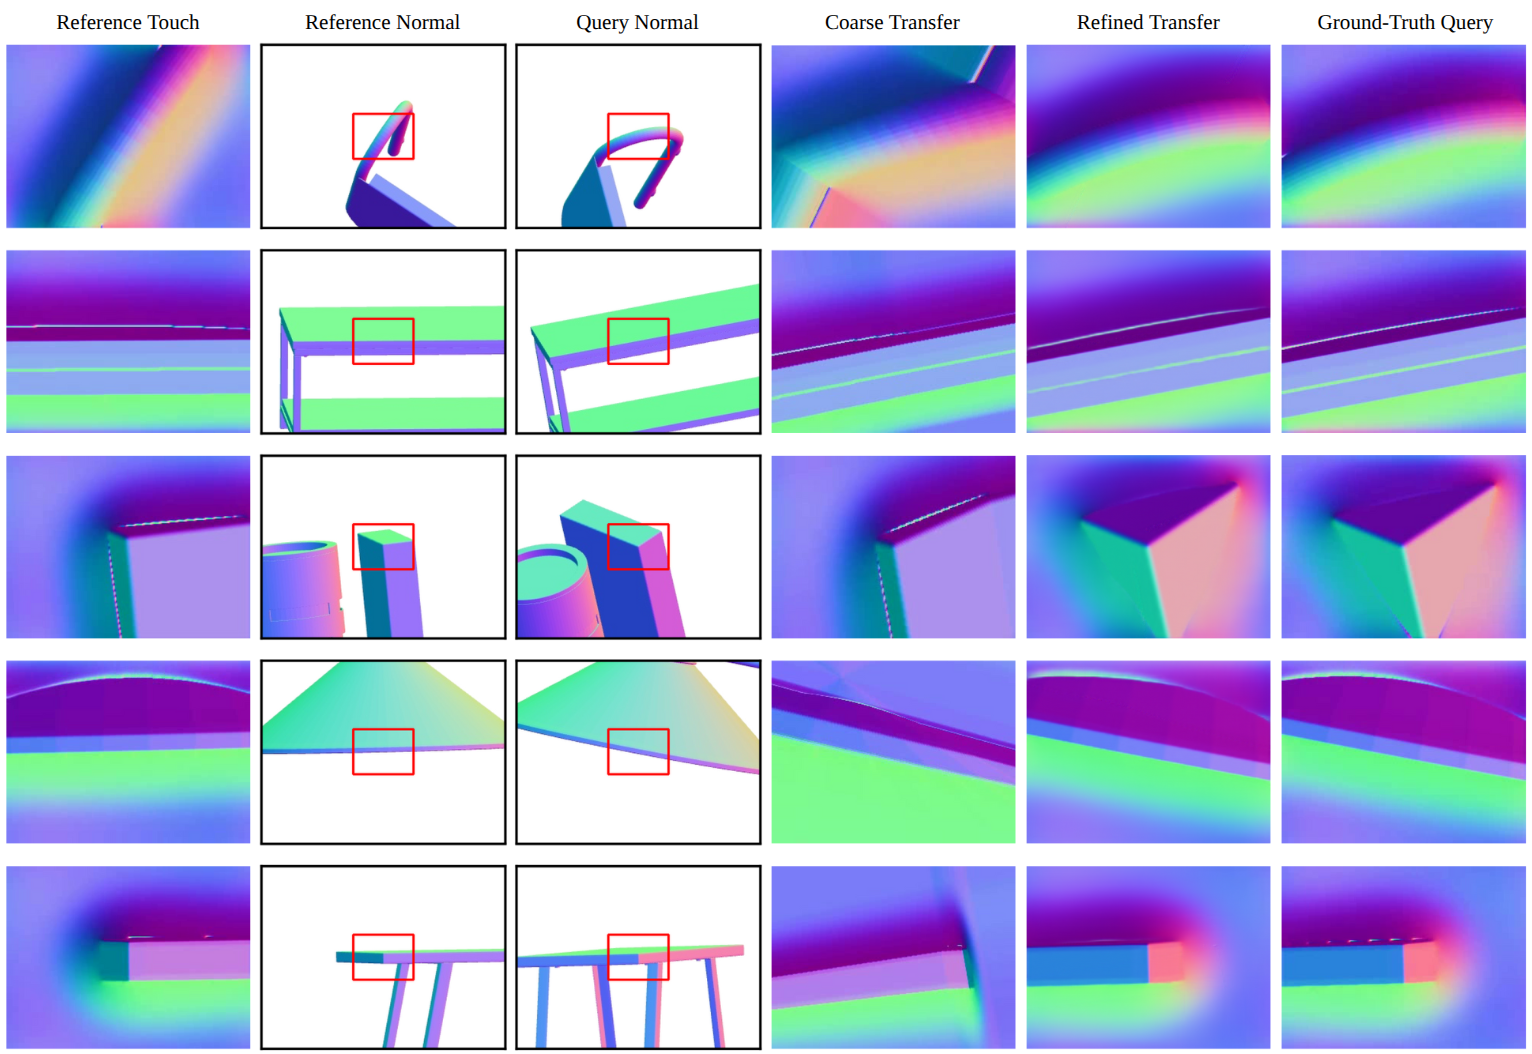
\includegraphics[width=\linewidth]{figures/gt_retrieval.png}
  \caption{\textbf{Qualitative results on the ground-truth retrieval benchmark.} Each row is one
    touch location. From left to right: the reference touch, the surface normal render at the
    reference sensor pose, the surface normal render at the query sensor pose, the coarse transfer
    obtained by warping the reference touch through the estimated homography, our refined
    prediction, and the ground-truth touch at the query location. The two normal renders cover
    four times the sensor footprint, which is the field of view the correspondences are computed
    at, and the red box marks the patch the sensor itself covers. All tactile frames are the
    middle frame of the 50-frame press, which is also the deepest-contact frame. The refinement
    network sharpens the contact boundary and corrects residual misalignment left by the coarse
    step.}
  \label{fig:gt_retrieval}
\end{figure*}


% TODO: finish writing the analysis once all baseline results are available.

\subsubsection{Full pipeline}

%% Full pipeline benchmark (retrieval + alignment + refinement): our method vs. baselines.
%% Numbers from paper_experiments/job2_full_pipeline/{results.md,table_body.tex}
%% (100 objects, 396 held-out query touches, 1121 reference touches).
\begin{table}[t]
  \centering
  \small
  \caption{\textbf{Full pipeline benchmark.} Prediction accuracy when retrieval is part of the
    evaluated system, averaged over all evaluation touches and all frames. ``Coarse'' is the
    transfer obtained from retrieval and feature-matching alignment alone, and ``refined''
    additionally applies the refinement network. Best result in \textbf{bold}.}
  \label{tab:full_pipeline}
  \begin{tabular}{l c c c}
    \hline
    Method & PSNR $\uparrow$ & SSIM $\uparrow$ & LPIPS $\downarrow$ \\
    \hline
    Tactile normal quilting~\cite{tactiledreamfusion} & 15.94 & 0.7145 & 0.4874 \\
    Implicit neural representation~\cite{objectfolder} & 21.11 & 0.8331 & 0.3769 \\
    \hline
    Ours (coarse transfer)                        & 21.60 & 0.7858 & 0.3304 \\
    Ours (refined)                                & \textbf{31.58} & \textbf{0.9182} & \textbf{0.1212} \\
    \hline
  \end{tabular}
\end{table}


Table~\ref{tab:full_pipeline} reports results on the full pipeline benchmark, which includes
retrieval error, again split into coarse and refined transfer.
Fig.~\ref{fig:full_pipeline} compares our predictions against the baselines frame by frame. Methods
that predict only a single image are shown with their prediction in the first column and marked
not applicable thereafter.

%% Qualitative comparison against the baselines on the full pipeline benchmark (two columns).
%% The graphic is a matrix of images:
%%   rows    -- one per method. The FIRST row shows the reference tactile normal video.
%%              Remaining rows: TaRF, tactile normal quilting, implicit neural representation,
%%              ours, ground truth.
%%   columns -- frames of the predicted video, sampled across the press.
%% For methods that predict a single image only, put the image in the first column and write
%% "N/A (image only)" in the remaining columns.
%% Replace the \rule placeholder below with the actual graphic.
\begin{figure*}[t]
  \centering
  % 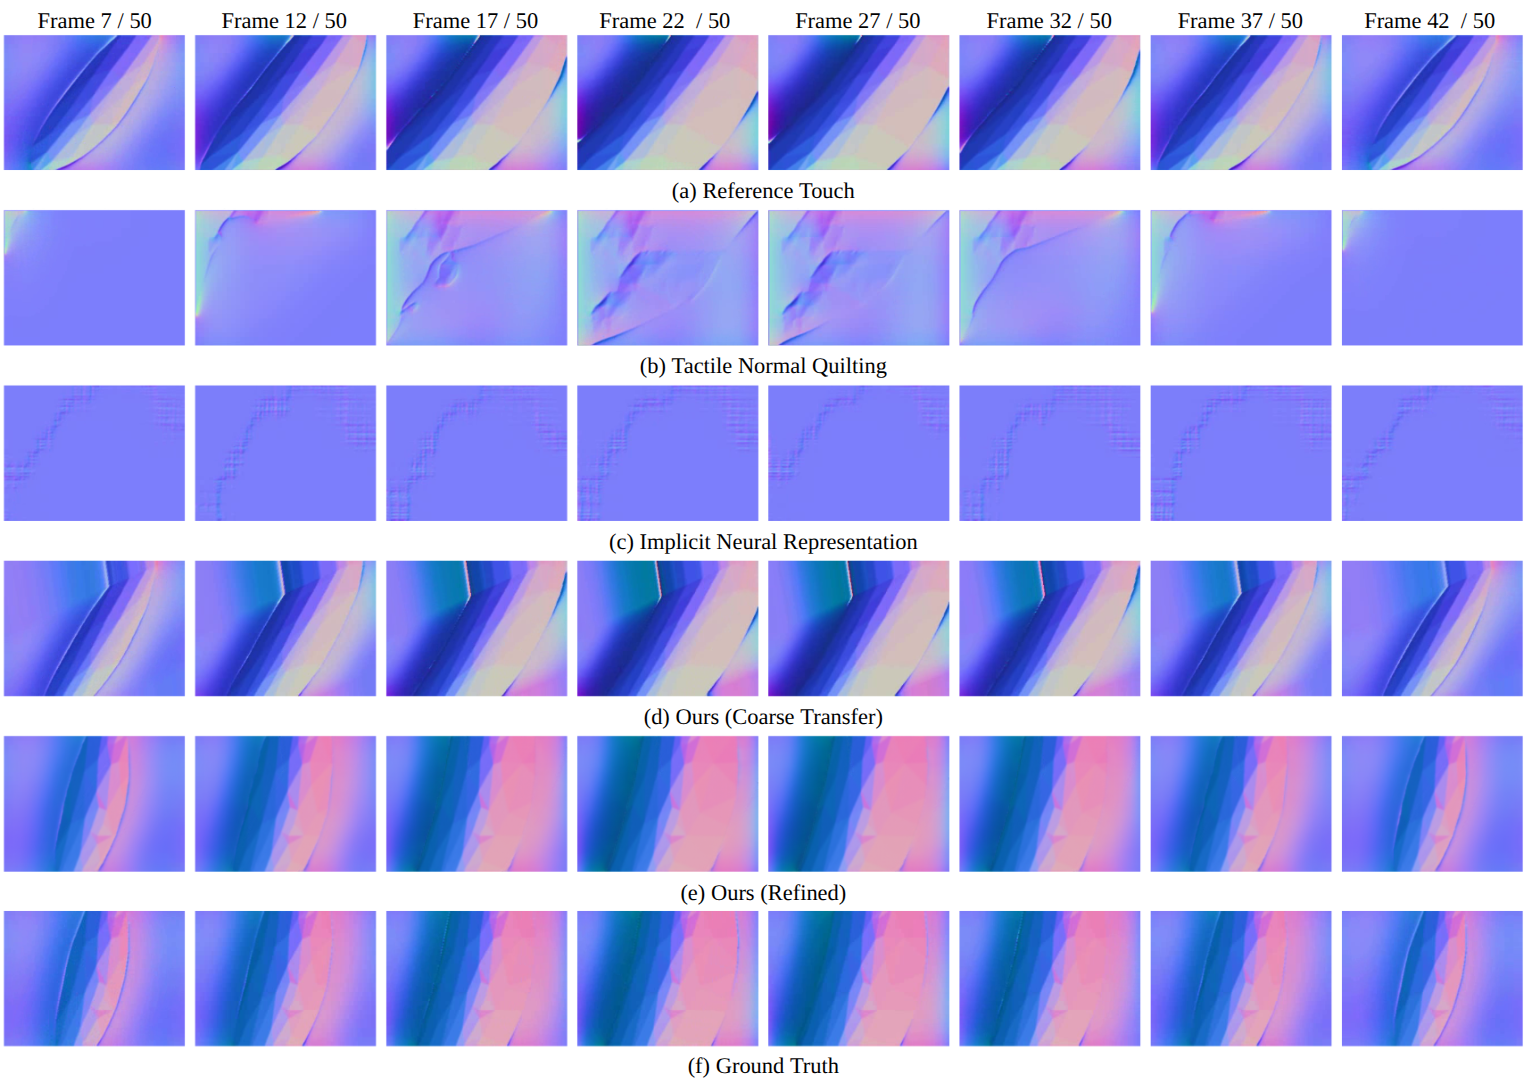
\includegraphics[width=\linewidth]{figures/full_pipeline_comparison.pdf}
  \rule{\linewidth}{7.0cm}% PLACEHOLDER -- remove when the real figure is dropped in
  \caption{\textbf{Comparison against baselines on the full pipeline benchmark.} Each row is one
    method and each column is a frame of the predicted tactile normal video, sampled across the
    press. The top row shows the reference tactile normal video that the prediction is transferred
    from. Baselines that predict a single tactile image rather than a video are shown with their
    prediction in the first column and marked \emph{N/A (image only)} thereafter, since they
    cannot express how the gel deforms over the press.}
  \label{fig:full_pipeline}
\end{figure*}


% TODO: finish writing the analysis once all baseline results are available.

\subsection{Ablation Study}

%% Ablation study on a 20-object subset of the full pipeline benchmark.
%% Cells are intentionally empty -- fill in the numbers.
\begin{table}[t]
  \centering
  \small
  \caption{\textbf{Ablation study} on a 20-object subset of the full pipeline benchmark. The top
    block varies the rendered modality used for retrieval and for feature matching, with the field
    of view fixed at $4\times$ the sensor footprint. The middle block varies that field of view,
    with the modality fixed to surface normals. The bottom block removes components of the
    refinement stage. The last row is our full model.}
  \label{tab:ablation}
  \begin{tabular}{l l c c c}
    \hline
    & Variant & PSNR $\uparrow$ & SSIM $\uparrow$ & LPIPS $\downarrow$ \\
    \hline
    \multirow{4}{*}{\rotatebox{90}{\scriptsize Modality}}
      & RGB              & & & \\
      & Height map       & & & \\
      & Curvature        & & & \\
      & Surface normals  & & & \\
    \hline
    \multirow{3}{*}{\rotatebox{90}{\scriptsize Scale}}
      & $1\times$        & & & \\
      & $2\times$        & & & \\
      & $4\times$        & & & \\
    \hline
    \multirow{4}{*}{\rotatebox{90}{\scriptsize Refinement}}
      & w/o neural refinement       & & & \\
      & w/o temporal FiLM           & & & \\
      & w/o normal concatenation    & & & \\
      & Ours (full)                 & & & \\
    \hline
  \end{tabular}
\end{table}


We ablate the key components of our method to show their contribution to accurate tactile
transfer. All ablations are run on a 20-object subset of the full pipeline benchmark, and
Table~\ref{tab:ablation} reports PSNR, SSIM and LPIPS. We study three groups of choices.

First, the \emph{modality} used for retrieval and for feature matching during initial alignment,
with the field of view fixed at $4\times$ the sensor footprint: surface normals (our default),
RGB colour, curvature, and height map. Second, the \emph{field of view} used for retrieval and
matching: $1\times$, $2\times$ and $4\times$. Third, the components of the refinement stage: no
neural refinement at all (i.e.\ the coarse transfer), no temporal FiLM conditioning, and no normal
map concatenation. Fig.~\ref{fig:ablation} compares predictions from the last three variants
visually.

%% Small qualitative ablation figure (one column). Graphic: figures/ablation_qualitative.png
%% 5 columns x 4 rows. Columns, left to right:
%%   ours w/o refinement (the coarse transfer) | ours w/o temporal FiLM |
%%   ours w/o normal concatenation | ours (full) | ground truth
%% Rows are four different query touch locations. Column headers are baked into the image.
\begin{figure}[t]
  \centering
  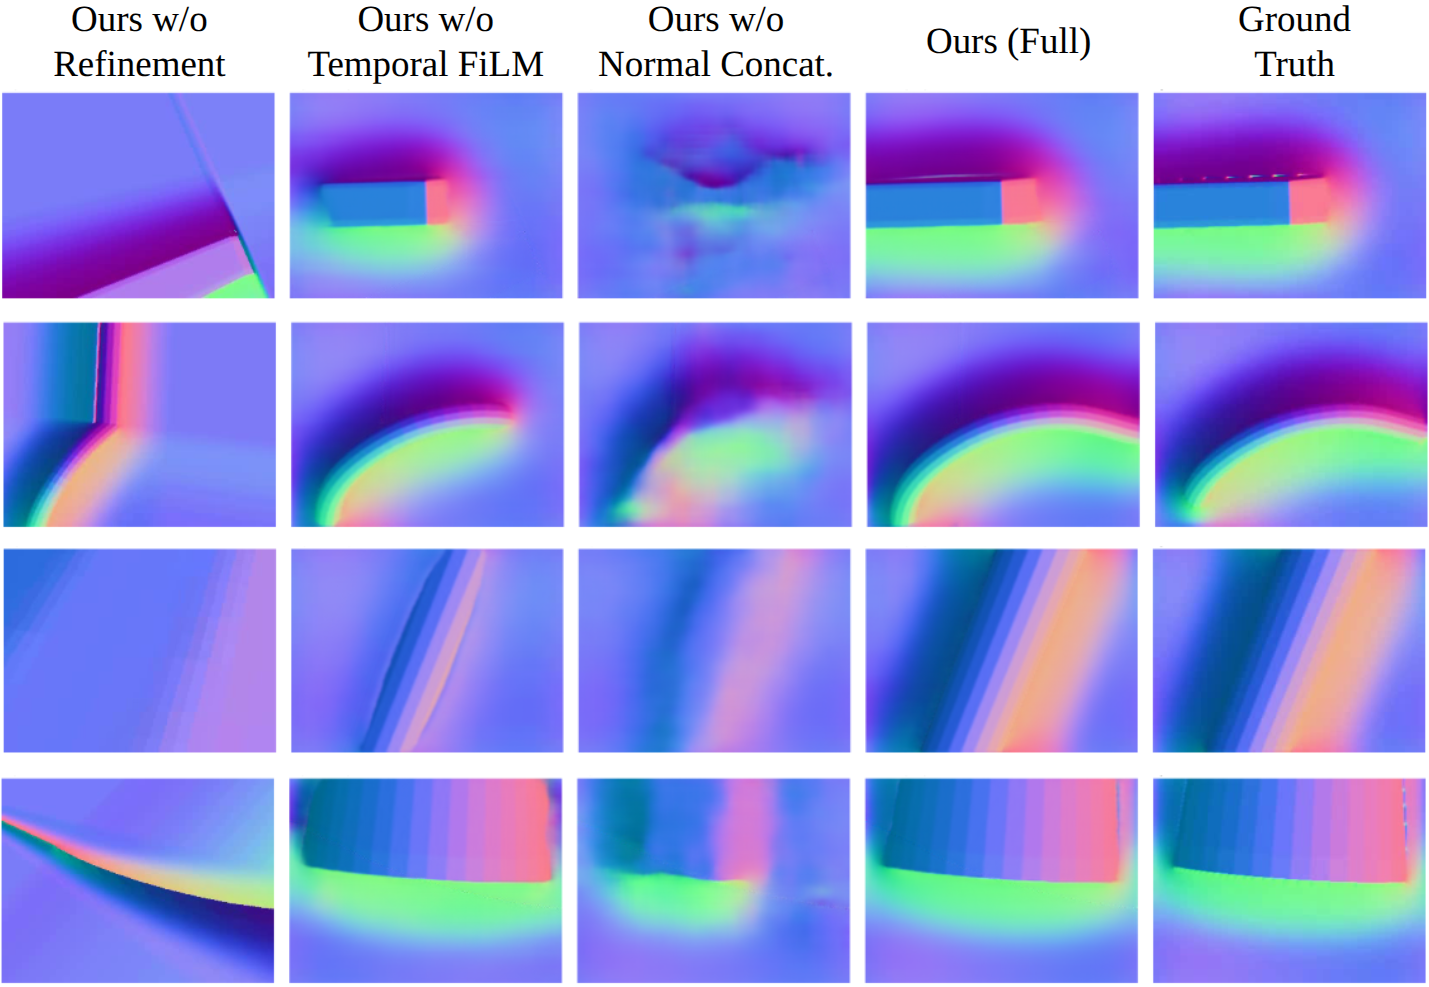
\includegraphics[width=\linewidth]{figures/ablation_qualitative.png}
  \caption{\textbf{Qualitative ablation of the refinement stage.} Each row is one query touch
    location, shown at the deepest-contact frame. From left to right: the coarse transfer with no
    neural refinement, refinement without temporal conditioning through FiLM, refinement without
    the concatenated query normal map, our full model, and the ground truth. Removing either
    conditioning signal degrades the prediction in a characteristic way. Without the query normal
    map the network has no evidence about the surface it is predicting for, and its output loses
    the contact geometry almost entirely. Without the timestamp the network cannot tell how deep
    into the press it is, so it recovers the shape of the contact but softens the edges that the
    full model keeps sharp.}
  \label{fig:ablation}
\end{figure}


% TODO: finish writing the analysis once all ablation results are available.

\subsection{Application in 3D Surface Reconstruction and Visuo-tactile Sensor Simulation}

%% 3D surface reconstruction and visuo-tactile sensor simulation (two columns).
%% The graphic is a matrix of images:
%%   row 1 -- reference tactile normal video (the example transferred from)
%%   row 2 -- predicted tactile normal video after refinement network inference
%%   row 3 -- 3D point cloud / shaded relief of the heightmap integrated from row 2, per frame
%%   row 4 -- RGB visuo-tactile video frames simulated from the same heightmap
%%   columns -- frames of the video, sampled from the in-contact portion of the press
%% Assets: log/paper_job03_recon_visuotactile/figure_951_5.png (alternates 977_1, 981_3,
%%         969_5, 967_1, 965_3).
%% Replace the \rule placeholder below with the actual graphic.
\begin{figure*}[t]
  \centering
  % \includegraphics[width=\linewidth]{figures/recon_visuotactile.pdf}
  \rule{\linewidth}{7.0cm}% PLACEHOLDER -- remove when the real figure is dropped in
  \caption{\textbf{3D surface reconstruction and visuo-tactile sensor simulation from predicted
    touches.} Columns are frames of a single press. Row~1: the reference tactile normal video the
    prediction is transferred from. Row~2: our predicted tactile normal video at the query
    location. Row~3: the 3D surface relief obtained by integrating the predicted normals into a
    heightmap with a Poisson solver. Row~4: the colour image a vision-based tactile sensor would
    have measured, simulated from the same heightmap with Taxim's calibrated optical model. Rows~3
    and~4 are deterministic post-processing of Row~2 and require no ground truth, so the whole
    chain runs at deployment time from a single reference touch. Frames are sampled from the
    in-contact portion of the press, since frames with no contact carry no signal to integrate.}
  \label{fig:recon}
\end{figure*}


Because our method predicts tactile surface normals rather than an opaque appearance signal, its
output can be turned into geometry with no additional supervision. We convert the predicted
normals into per-pixel surface slopes and integrate them into a heightmap with a Poisson solver,
subtracting a least-squares plane fit since the integration is defined only up to a plane. The
result is a 3D reconstruction of the object surface at a location that was never physically
touched. Such reconstructions let an embodied agent reason about fine-grained shape properties of
previously untouched regions, and can drive haptic rendering.

Going one step further, feeding the same heightmap through Taxim's calibrated optical
model~\cite{taxim} produces the colour image a camera-based tactile sensor would have measured ---
a virtual visuo-tactile measurement. This could aid manipulation policies that are trained
directly on visuo-tactile sensor readings: an agent could, for instance, rehearse a grasp by
predicting the tactile videos at candidate contact points before touching the object at all.
Fig.~\ref{fig:recon} shows the full chain, from reference touch through predicted tactile normal
video to the reconstructed 3D relief and the simulated colour frames. Both steps after the network
are deterministic post-processing of the predicted normals, so the whole chain runs at deployment
time from a single reference touch.

\subsection{Runtime Analysis}

We report the runtime of our full pipeline, measured on an RTX 3090 GPU. Given $N$ reference
touches and one query, producing a touch prediction takes \tbd{}\,s for the retrieval phase after
DINOv3 feature extraction, \tbd{}\,s for coarse alignment after local feature matching, and
\tbd{}\,s per frame for neural refinement. Thanks to these short runtimes our method is lightweight and
well suited to runtime-critical applications such as AR/VR and robotics.
